\documentclass[border=10pt]{standalone}
\usepackage{tikz}
\usepackage{amsmath}	% Advanced maths commands
\usetikzlibrary{arrows.meta}

\begin{document}    
	\centering
	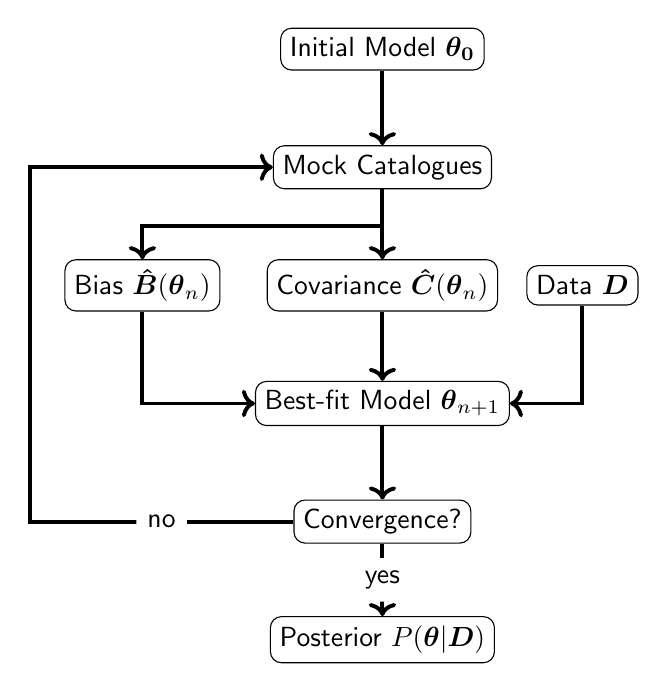
\begin{tikzpicture}[node distance=1.5cm, every node/.style={rounded corners, fill=white, draw=black, font=\sffamily}, align=center, minimum height=0.5cm]
	% Specification of nodes (position, etc.)
	\node (InitialModel)	[]								{Initial Model $\boldsymbol{\theta_0}$};
	\node (Mocks)			[below of=InitialModel]			{Mock Catalogues};
	\node (ModelBias)		[below of=Mocks, xshift=-1.2in]	{Bias $\boldsymbol{\hat{B}}(\boldsymbol{\theta}_{n})$};
	\node (Covariance)		[below of=Mocks]				{Covariance $\boldsymbol{\hat{C}}(\boldsymbol{\theta}_{n})$};
	\node (Data)			[below of=Mocks, xshift=1.0in]	{Data $\boldsymbol{D}$};
	\node (NewModel)		[below of=Covariance]			{Best-fit Model $\boldsymbol{\theta}_{n + 1}$};
	\node (Convergence)		[below of=NewModel]				{Convergence?};
	\node (Posterior)		[below of=Convergence]			{Posterior $P(\boldsymbol{\theta} | \boldsymbol{D})$};
	\draw[->, line width=0.5mm]	(InitialModel) -- (Mocks);
	\draw[->, line width=0.5mm]	(Mocks) -- ++(0, -0.75) -| (ModelBias);
	\draw[->, line width=0.5mm]	(Mocks) -- (Covariance);
	\draw[->, line width=0.5mm]	(ModelBias.south) |- (NewModel.west);
	\draw[->, line width=0.5mm]	(Covariance) -- (NewModel);
	\draw[->, line width=0.5mm]	(Data.south) |- (NewModel.east);
	\draw[->, line width=0.5mm]	(NewModel) -- (Convergence);
	\draw[->, line width=0.5mm]	(Convergence) -- node[draw=white]{yes}(Posterior);
	\draw[->, line width=0.5mm] (Convergence.west) -- node[draw=white]{no} ++(-3.35,0) |- (Mocks.west);
	\end{tikzpicture}
\end{document}